
\documentclass[conference]{IEEEtran}
\usepackage{blindtext, graphicx}
\usepackage{listings}
\usepackage{framed}
\usepackage{caption}
\usepackage{float}
\usepackage{tikz, pgfplots}


\ifCLASSINFOpdf
\else
\fi

% correct bad hyphenation here
\hyphenation{}

\usepackage{bera}% optional: just to have a nice mono-spaced font
\usepackage{listings}
\usepackage{xcolor}

\colorlet{punct}{red!60!black}
\definecolor{background}{HTML}{EEEEEE}
\definecolor{delim}{RGB}{20,105,176}
\colorlet{numb}{magenta!60!black}

\lstdefinelanguage{json}{
    basicstyle=\ttfamily\normalfont\footnotesize,
    numbers=left,
    numberstyle=\scriptsize,
    stepnumber=1,
    numbersep=9pt,
    showstringspaces=false,
    breaklines=true,
    frame=lines,
    backgroundcolor=\color{background},
    literate=
     *{0}{{{\color{numb}0}}}{1}
      {1}{{{\color{numb}1}}}{1}
      {2}{{{\color{numb}2}}}{1}
      {3}{{{\color{numb}3}}}{1}
      {4}{{{\color{numb}4}}}{1}
      {5}{{{\color{numb}5}}}{1}
      {6}{{{\color{numb}6}}}{1}
      {7}{{{\color{numb}7}}}{1}
      {8}{{{\color{numb}8}}}{1}
      {9}{{{\color{numb}9}}}{1}
      {:}{{{\color{punct}{:}}}}{1}
      {,}{{{\color{punct}{,}}}}{1}
      {\{}{{{\color{delim}{\{}}}}{1}
      {\}}{{{\color{delim}{\}}}}}{1}
      {[}{{{\color{delim}{[}}}}{1}
      {]}{{{\color{delim}{]}}}}{1},
}

\usepackage{lmodern}
\usepackage[utf8]{inputenc}
\usepackage[russian,english]{babel} % last one is the main language
\selectlanguage{english}

\newenvironment{russian}{
\begin{otherlanguage*}{russian}
}{
\end{otherlanguage*}
}

% URL
\usepackage{hyperref}
\urlstyle{tt}

% Better discription
\usepackage{enumitem}

%bib


\begin{document}
%
% paper title
% can use linebreaks \\ within to get better formatting as desired
\title{ICLab Collateral Censorship}


% author names and affiliations
% use a multiple column layout for up to three different
% affiliations
\author{\IEEEauthorblockN{Jesse Brizzi}
\IEEEauthorblockA{jbrizzi@cs.stonybrook.edu}
\and
\IEEEauthorblockN{Konstantin Dmitriev}
\IEEEauthorblockA{kdmitriev@cs.stonybrook.edu}
\and
\IEEEauthorblockN{Yingtao Tian}
\IEEEauthorblockA{yittian@cs.stonybrook.edu}
}

% make the title area
\maketitle


\begin{abstract}
%\boldmath
In this project we are proposing a survey of neighboring sovereign nations to modern day Russia to investigate any possible collateral censorship.
Given the socioeconomic state of some of these countries there may be limited infrastructure for Internet access, which requires their traffic to be routed through Russian territory.
Russia actively censors various websites and Internet sources based on various reasons.
We intend to use this to fulfill the experiment portion of project option 1 in the class forking the IClab software to complete our experiment. 
As part of option 1 we will also create a Web interface to run our experiment on IClab and a website presenting our final results.

\end{abstract}
% IEEEtran.cls defaults to using nonbold math in the Abstract.
% This preserves the distinction between vectors and scalars. However,
% if the journal you are submitting to favors bold math in the abstract,
% then you can use LaTeX's standard command \boldmath at the very start
% of the abstract to achieve this. Many IEEE journals frown on math
% in the abstract anyway.

% Note that keywords are not normally used for peerreview papers.
\begin{IEEEkeywords}
Collateral Censorship, Russia, Block, DPI, DNS, IP.
\end{IEEEkeywords}

% For peerreview papers, this IEEEtran command inserts a page break and
% creates the second title. It will be ignored for other modes.
\IEEEpeerreviewmaketitle



\section{Motivation}
In the summer of 2008, when Russia's mass media and telecom watchdog Roskomnadzor \footnote{Federal Service for Supervision of Communications, Information Technology and Mass Media (Russian:
\begin{russian}Федеральная служба по надзору в сфере массовых коммуникаций и связи\end{russian}
)} was re-established, the Russian Internet, or RuNet, changed  significantly. 
This Federal Service is regulated and put into motion by two laws, - ``On Protecting Children from Information Harmful to Their Health and Development''\cite{krem1} and ``On Information, Information Technology and Information Protection''\cite{krem2}. 
Both of them give judges a free hand in decision-making. As a result, a number of websites have been blocked quite chaotically, starting with opposition websites and articles, to Bitcoin communities and GitHub.

\indent Sometimes such censorship systems can case collateral censorship, or damage. 
They block access to sites from users beyond those intended to protect\cite{anon1}. 
This projects goal is to examine the effect of such possible collateral censorship to the requests that are originating from outside of Russia, with the possible extension to other countries that maintain the censoring services. 
The result of this project can be used to create a detailed analysis of collateral damage caused by different types of censoring techniques, and to potentially discover the paths at fault.

\section{Censorship tools}
The Russian Internet Service Providers (ISPs) and government use a number of different censorship techniques to block access to ``unwanted'' websites. 
Fig. \ref{fig:fig1} shows a chart of the most popular ones by the number of providers that maintain a particular method.
\begin{figure}[H]
\centering
\begin{tikzpicture}
\begin{axis}[
    ybar,
    enlargelimits=0.15,
    legend style={at={(0.5,-0.15)},
      anchor=north,legend columns=-1},
    ylabel={\#providers},
    symbolic x coords={DPI-IP, IP, DPI-FULL, DNS},
    xtick=data,
    nodes near coords, 
	nodes near coords align={vertical},
    x tick label style={rotate=45,anchor=east},
    xlabel={Blocking Method},
    x label style={at={(0.5,-0.25)}}
    ]
\addplot coordinates {(DPI-IP,430) (IP,235) (DPI-FULL,125) (DNS, 155)};
\end{axis}
\end{tikzpicture}
\caption{Number of providers that maintain a particular blocking method (DPI-IP - blocking using Deep Packet Inspection (DPI), that checks URL only at a specific IPs and port:80; DPI-FULL - blocking using DPI at every IP and ports; IP - blocking by IP address; DNS - DNS injection)}
\label{fig:fig1}
\end{figure}

\section{Resources}
\indent As a main reference for blacklisted URLs, domain names, and IPs in Russia, we plan to use the service \url{http://antizapret.info} which maintains and persistently updates its catalog. 
In addition, it also provides an API for external access. 

\begin{lstlisting}[language=json,firstnumber=1,caption={An example of the possible output from requesting
\url{http://api.antizapret.info/all.php?type=json}}, label=listing1, frame=single] 
"id":"16971",
"rsoc_id":"91191193",
"includeTime":"2015-02-13 11:55:47",
"rsocDate":"2015-02-04",
"org":"",
"org_act":"2/1/11-32425",
"url":http://chetkiibro.com/,
"domain":"http://chetkiibro.com/,
"ip":"104.28.16.89,104.28.17.89",
"country":"",
"proof":"http://antizapret.info/site.php?id=16971"
\end{lstlisting}
As a reference of the potential victims of the collateral censorship, we are going to use telegraphy maps (Fig. \ref{fig:fig3}), and the map of the supported countries for one of the largest Russian backbone service provider (Fig. \ref{fig:fig2}), concentrating on the bordering countries. 

\begin{figure}[H]
\centering
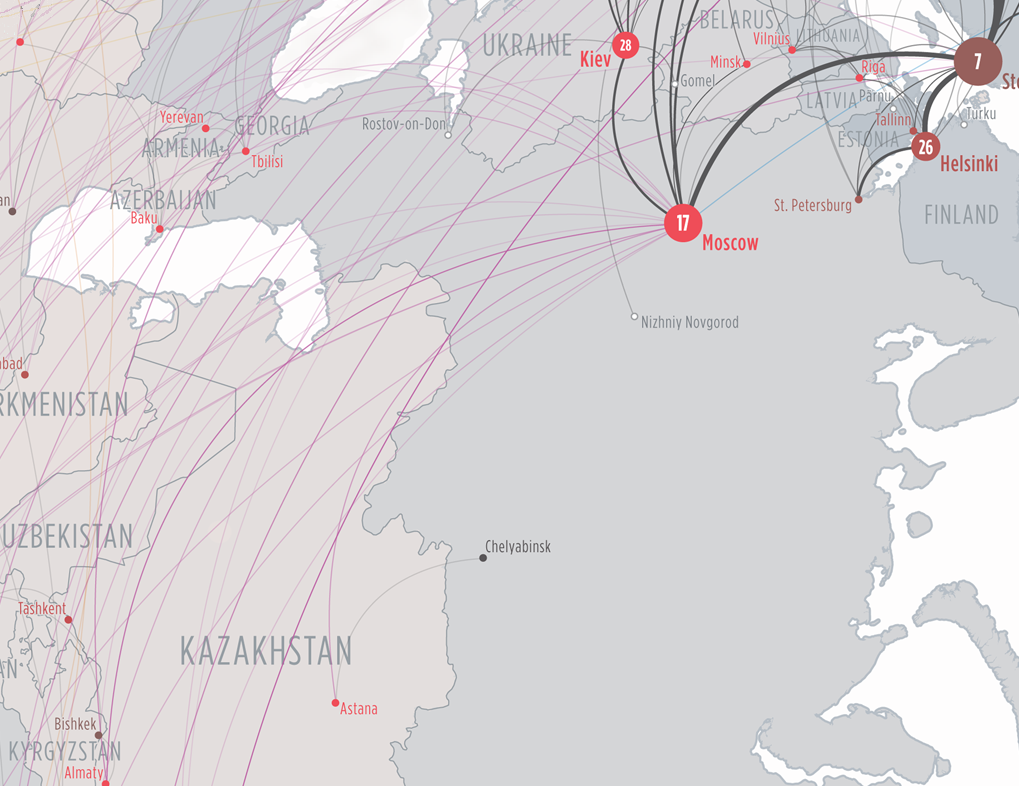
\includegraphics[width=.45\textwidth]{routeMap.png}
\caption{Telegeography Map of the Region \label{teleG}}
\label{fig:fig3}
\end{figure}

\begin{figure}[H]
\centering
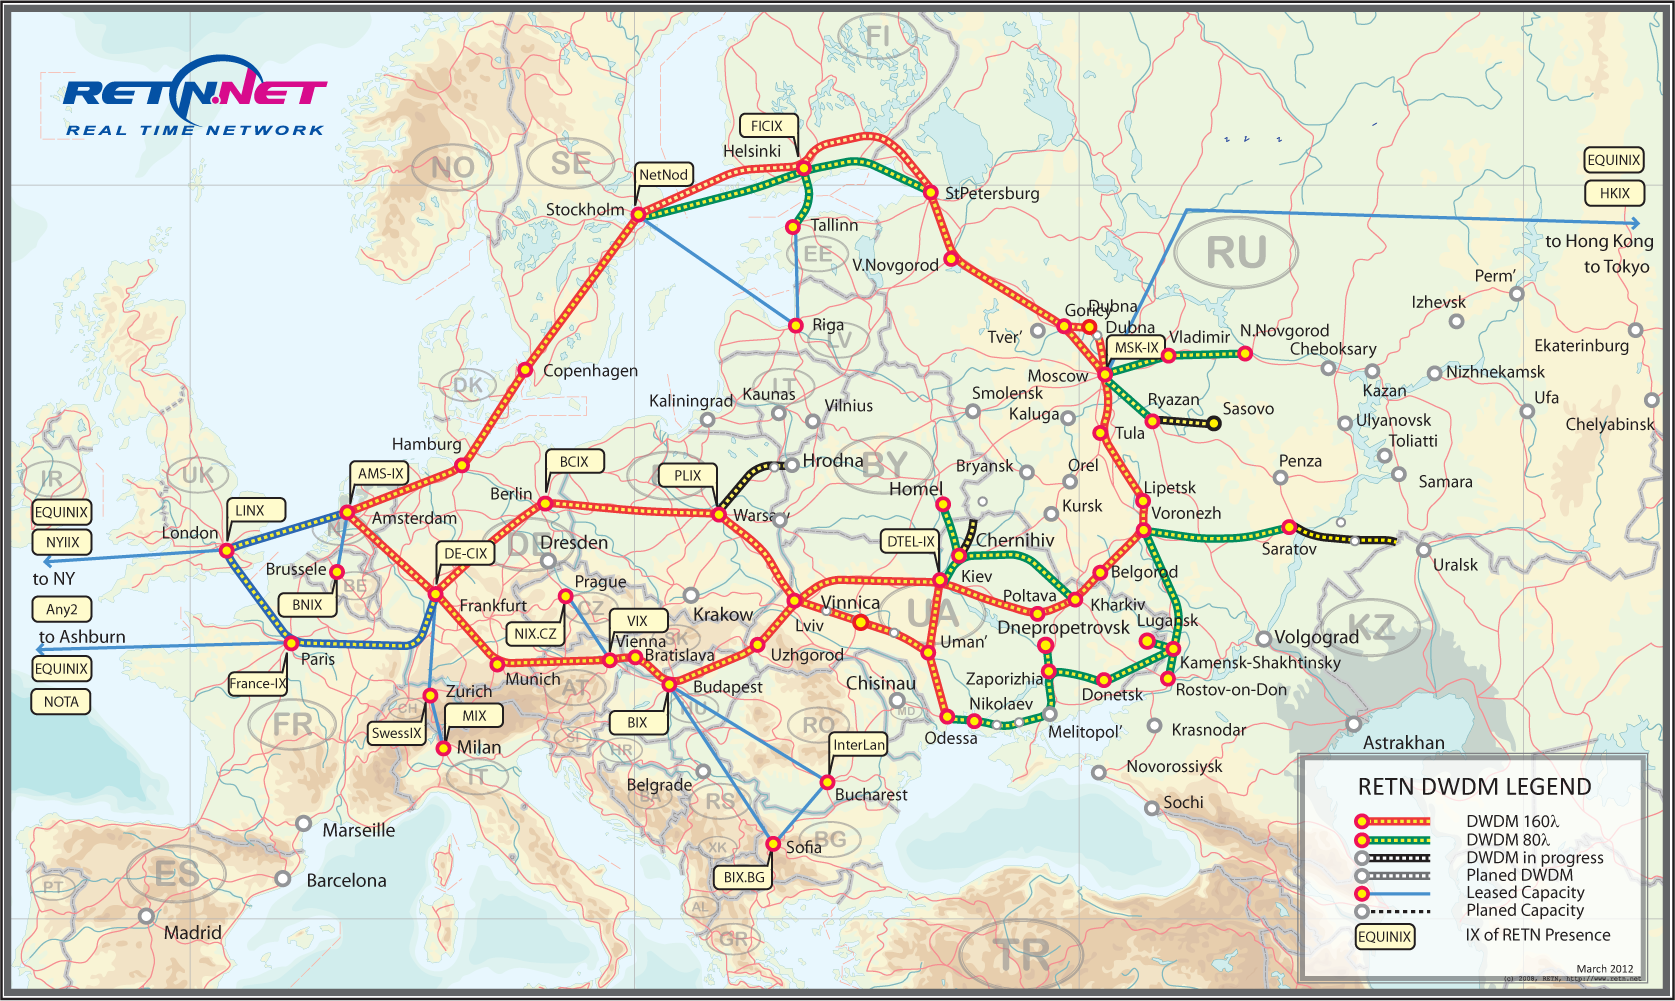
\includegraphics[width=85mm]{figure2.png}
\caption{RETN's backbone map \label{RetnMap}}
\label{fig:fig2}
\end{figure}


\section{Research Plan}
\subsection{Ultimate Plan(?)}
Our ultimate aim is to write an experiment for the ICLab project \cite{IClab} in the form of Python scripts that will probe websites censored in Russia from computers of registered ICLab users. 
This experiment will not only be able to compare the received web-pages with the blocked ones, but also return the type of the applied censorship technique in case of detected similarity between the received and the blocked web-pages. 
To collect the source code of blocked web-pages we plan to use our groups own private computer in Russia or a VPN service

In order to create this experiment, we plan to use the following modules:
\begin{enumerate}
\item \textbf{urllib} - for network resource access;
\item \textbf{socket} - to get an access to the BSD socket interface;
\item \textbf{ssl} - to get an access to Transport Layer Security encryption and peer authentication facilities for network socket;
\item \textbf{dnspython} - to get an access to high and low levels of DNS. 
\end{enumerate}

The coarse description of the experiment is the following:
\begin{enumerate}
\item Collect a list of URLs and IPs of the censored web-pages from \url{http://antizapret.info};
\item For each item in the list:
    \begin{enumerate}
    \item Request the web-page and compare its source code with the code of actually blocked web-page;
    \item Test DNS access;
    \item Test HTTP access.
    \end{enumerate}
\end{enumerate}

\subsection{Contingency Plan}
Given the possibility where no censorship leakage is found, we will restructure the experiment to try and prove our results are accurate, i.e.\  that there is little to no collateral censorship resulting from the Russian government. 
This will be done by repeating the experiment multiple times at different times of the day, along with expanding our list of candidates for possible collateral censorship to other countries in close proximity geographically and in terms of Internet topology. 

\section{Web User Interface}
To display the results of our tests we will create a Web UI, that will consists of a table with the outcomes of the particular experiment, including URL addresses, URL categories, statuses and explanations. That Web UI will also have an option that will give the user a visual summary for the all conducted experiments. 

\section{Timeline}
Estimation of progress by week.

\begin{description}[leftmargin=6em,style=nextline]
\item[2/16 - 2/22] Setup and design
\item[2/23 - 3/01] Design Interface Website/Experiment
\item[3/02 - 3/08] Code Interface Website/Experiment
\item[3/09 - 3/15] Code Interface Website/Experiment
\item[3/16 - 3/22] Spring Break/Coding/Debugging
\item[3/23 - 3/29] Run Experiment
\item[3/30 - 4/05] Run Experiment/Analysis Data
\item[4/06 - 4/12] Midterm project Report due
\item[4/13 - 4/19] Expand Experiment if needed
\item[4/20 - 4/26] Create Website for Results
\item[4/27 - 5/03] Buffer Week
\item[5/04 - 5/10] Final Project Report Due
\end{description}


\begin{thebibliography}{9}


\bibitem{anon1}
  Anonymous,
  \emph{The Collateral Damage of Internet Censorship by DNS Injection}.
  SIGCOMM Comput. Commun. Rev., July 2012.
  
\bibitem{krem1}
    \emph{"Law on Protecting Children from Negative and Harmful Information."} President of Russia. N.p., n.d. Web. 14 Feb. 2015. 
    
\bibitem{krem2}
    \emph{Russian Federation: Federal Law No. 149-FZ} of July 24, 2006, on Information, Information Technology and Information Protection (as Amended up to Federal Law No. 398-FZ of December 28, 2013). N.p., n.d. Web. 14 Feb. 2015.
    
\bibitem{IClab}
    \emph{ICLab}. GitHub. N.p., n.d. Web. 15 Feb. 2015. https://github.com/iclab.

\end{thebibliography}

\end{document}


